\section{Experimental results}
\label{sec:experimental_results}
The proposed hardware/software co-design framework is demonstrated on XC7Z007S with 1 TP instance, and XC7Z010 with 2 TP instances. On the PL, we implement the proposed hardware architecture with a clock frequency at $200 MHz$. On the PS, we execute the bare-metal software architecture on the ARM Cortex-A9 at $666MHz$ in both devices.

To demonstrate the proposed design, we build models $A$ and $B$ in TensorFlow. Model $B$ incorporates depthwise separable convolution operations (a depthwise convolution followed by a pointwise convolution). See \Fig{fig:models}.

\begin{figure}[t!]
	\centering
	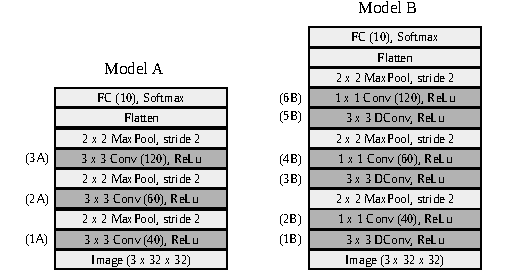
\includegraphics[width=0.5\textwidth]{../figures/models.pdf}
	\caption{Shallow CNN models for case study.}
	\label{fig:models}
\end{figure}

\subsection{Custom floating-point format based on classification accuracy}
To obtain the best number format, we train $A$ and $B$ with CIFAR-10 using early stop and batch size of 20, and \emph{adam} optimizer. The proposed quantized-aware training method is used with two iterations, see \fig{fig:accuracy}.

To demonstrate hardware feasibility, $A$ and $B$ are evaluated by addressing a design exploration with hybrid custom floating-point and hybrid logarithmic approximation. We explore three reduced floating-point formats for filter and bias: exponent $E_{size} = 5, 4, 3$-bits, all formats with mantissa $M_{size} = 1$-bit and sign $S_{size} = 1$-bit. For Logarithmic approximation, we remove the mantissa bit.

\begin{figure}[t!]
	\centering
	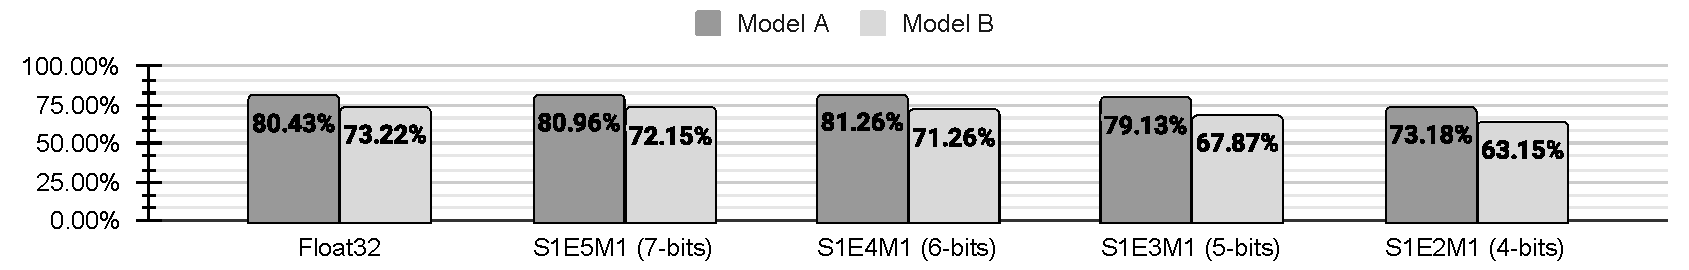
\includegraphics[width=0.5\textwidth]{../figures/all_models_accuracy.pdf}
	\caption{Accuracy performance using the proposed training method.}
	\label{fig:accuracy}
\end{figure}


\subsection{Hardware design exploration}
To evaluate the methodology, we employ \Equ{eq:channel_in_memory}, giving the maximum hyper parameters from models $A$ and $B$: $W_{I}=32$, $C_{I}=60$, $C_{O}=120$, $K_{W} = K_{H} =3$. For the number formats, $BitSize_{I}=32$-b, and $BitSize_{F} = BitSize_{B}=6$-bits. To determine $V_{M}$, we use HLS tool, which gives an estimate of 6 RAM blocks. The performance evaluation and the hardware resource utilization are displayed in \tab{tab:perf} and \tab{tab:resource}, respectively.

\begin{enumerate}
\item{\textbf{XC7Z007S}}: As a resource-limited FPGA, this device has a capacity of 14,400 LUTs and 1.8Mb of BRAM. This limitation allows to instantiate one TP with \emph{Conv} due to its LUT capacity. With \Equ{eq:tp_memory}, we obtain a BRAM utilization of 789.84Kb. This implementation presents a peak runtime acceleration of $55\times$ in model $A$ at the tensor operation \emph{(3A) Conv} with a power reduction of $808\times$.

\item{\textbf{XC7Z010}}: This device has a capacity of 17,600 LUTs and 2.1Mb of BRAM. These resources allow to instantiate two TPs with \emph{Conv}, and one TP with \emph{Conv} and \emph{DConv} engines. With \Equ{eq:tp_memory}, we obtain a BRAM utilization of 1,580Kb. This implementation presents a peak runtime acceleration of $105\times$ in model $A$ at the tensor operation \emph{(3A) Conv} with a power reduction of $1121\times$. On model $B$, \emph{(6B) Conv} presents a peak acceleration of $43.8\times$. The \emph{DConv} tensor operator yields an acceleration of $6.75 \times$, which is limited since the pipelined vector dot-product performs on channel wise.
\end{enumerate}

\begin{table}[!h]\centering
	\caption{Hardware resource utilization and estimated power dissipation.}\label{tab:resource}
	\scriptsize
	\begin{tabular}{lrrrrrrr}\toprule
		\multirow{2}{*}{\textbf{Device}} &\multirow{2}{*}{\textbf{TP}} &\multicolumn{4}{c}{\textbf{Post-implementation resource utilization}} &\multirow{2}{*}{\textbf{Power (W)}} \\\cmidrule{3-6}
		& &\textbf{LUT} &\textbf{FF} &\textbf{DSP} &\textbf{BRAM 36Kb} & \\\midrule
		\multirow{2}{*}{XC7Z007S} &\multirow{2}{*}{1} &7,939 &8,955 &20 &25 &\multirow{2}{*}{1.44} \\
		& &55\% &31\% &30\% &50\% & \\\midrule
		\multirow{2}{*}{XC7Z010} &\multirow{2}{*}{2} &13,542 &15,279 &36 &46 &\multirow{2}{*}{1.880} \\
		& &77\% &43\% &45\% &76\% & \\
		\bottomrule
	\end{tabular}
\end{table}
